\documentclass[twocolumn]{article}
\usepackage{graphicx}
\usepackage{amsmath}
\usepackage{booktabs}
\usepackage{multicol}
\usepackage{multirow}
\usepackage[margin = 2cm]{geometry}
\usepackage{array}
\usepackage{xcolor}

\begin{document}

\begin{titlepage}
    \centering
    \vspace*{-2cm}
    
\includegraphics[width=0.4\textwidth]{UoM.jpg}
    \vspace{1.5cm}

    {\LARGE University of Moratuwa}\\[0.5cm]
    {\large Department of Electronic \& Telecommunication Engineering}\\[2cm]
    
    {\Large EN2160 - Electronic Design Realization}\\[0.5cm]
    {\Large Report}\\[1.5cm]
    
    \textbf{\Large Simple Solar Battery Charger}\\[1cm]
    \textbf{\Large Efficient Charging Solution for Outdoor Activities}\\[1cm]
    
    \begin{minipage}{0.4\textwidth}
        \begin{flushleft}
        \centering
            \textbf{\large Ahamed M.B.S.A. – 200014B}\\
        \end{flushleft}
    \end{minipage}
    
    \vfill
    
    {\large THIS REPORT IS SUBMITTED IN PARTIAL FULFILLMENT OF THE REQUIREMENTS FOR THE MODULE}\\[0.5cm]
    {\large EN2160 - Electronic Design Realization}\\[0.5cm]
    {\large 16th of June 2023}
    
\end{titlepage}

\begin{abstract}
    A simple solar battery charger is a compact and portable device designed to harness solar energy and convert it into electrical energy for charging rechargeable batteries. With the increasing demand for renewable energy solutions, solar panels have gained popularity as a reliable source of power. However, due to the variable nature of sunlight intensity and environmental conditions, it is crucial to have an effective solar controller to regulate the charging process safely. This charger uses LM338 or LM317 as the solar controller to ensure consistent and safe charging of batteries. Additionally, two LEDs are incorporated to indicate the battery charge level, making it easy to monitor and maintain the battery.
\end{abstract}

\section*{Introduction}
    \subsection*{1. Problem Validation}
    Traditional battery chargers often rely on an   alternating current (AC) power source, which can be challenging to access in remote locations or during power outages. Moreover, these chargers may lack the capability to efficiently utilize solar energy due to the variable nature of sunlight intensity and other environmental factors. The problem is to design a simple solar battery charger that effectively manages the charging process, optimizing the use of solar power while ensuring the safety and longevity of the connected batteries.
    \vspace{5pt}
    
    \noindent To tackle this problem, the charger incorporates LM338 or LM317 as the solar controller, providing a reliable mechanism to regulate the charging voltage and current. This control is crucial to prevent overcharging, which could damage the batteries, and to optimize charging efficiency based on the available sunlight.
    
    \subsection*{2. Problem Description}
    The need for a simple solar battery charger is validated by the increasing demand for portable and eco-friendly charging solutions. As solar panels have become more accessible and affordable, their adoption for various applications has grown significantly. The challenge lies in ensuring that the solar charging process is stable, efficient, and suitable for a wide range of battery capacities.
    \vspace{5pt}
    
    \noindent By incorporating LEDs to indicate battery charge levels and using solid-state design without relays, the charger provides an easy way to monitor the charging status, making it user-friendly and suitable for outdoor use. Additionally, the charger's water-resistant and heat-resistant properties ensure durability and reliability in diverse environmental conditions, further validating its practicality.
    \vspace{5pt}
    
    \noindent With its cost-effectiveness, lightweight design, and compatibility with different battery capacities, the simple solar battery charger addresses the problem of sustainable charging during outdoor activities, making it a compelling solution for individuals seeking an alternative to traditional AC-powered chargers in off-grid or power-constrained scenarios.

\section*{Compoeents}
We use basic electronic components to build the PCB to work with this system.

\subsection*{1. LM317T Regulator:}

The LM317T is a versatile regulator IC that can be used to step down voltages efficiently. In this case, we will configure it as an adjustable voltage regulator to obtain the desired 4.2V output for charging the 3.7V battery.

\subsection*{2. 1N4731 Zener Diode (3.7V):}

We will use the 3.7V Zener diode in conjunction with the LM317T to provide a stable voltage reference. The Zener diode will act as a voltage shunt regulator, helping to maintain the output voltage at a constant level.
\vspace{10pt}

\noindent \textbf{ Step-by-Step Conversion Process:}
\vspace{5pt}

\begin{enumerate}
    \item Connect the input of the LM317T regulator to the output of the 5V solar panel.
    
    \item Place the Zener diode between the output (Vout) and the adjustment (ADJ) pin of the LM317T.
    
    \item Adjust the resistor network of the LM317T to set the output voltage to approximately 4.2V. This can be done by calculating the resistor values using the LM317T datasheet or by using an online LM317T voltage calculator.
    
    \item Ensure the total power dissipation of the Zener diode and LM317T does not exceed their respective ratings to avoid overheating.
    
    \item Connect the regulated output (approximately 3.7V) to the 3.7V battery for charging.
\end{enumerate}

\subsection*{3. Other Components}
listed the other components we have used except the components listed above.
\vspace{5pt}

\begin{table}[ht]
    \centering
    \caption{Component Values and Quantities}
    \begin{tabular}{|l|l|c|}
        \hline
        \textbf{Component} & \textbf{Value} & \textbf{Quantity} \\
        \hline
        Switch & & 1 \\
        \hline
        Resistor & 2.2 K$\Omega$ & 1 \\
        \hline
        Resistor & 1 K$\Omega$ & 5 \\
        \hline
        Resistor & 240 $\Omega$ & 1 \\
        \hline
        Preset resistor & 1 K$\Omega$ & 1 \\
        \hline
        IN 4007 diode & & 2 \\
        \hline
        1N4731 Zener diode & 3.7V & 1 \\
        \hline
        Li-ion Battery & 3.7V & 4 \\
        \hline
        Transistor & BD 139 & 1 \\
        \hline
        LED & Red & 1 \\
        \hline
        LED & Green & 1 \\
        \hline
        Battery Case & & 1 \\
        \hline
    \end{tabular}
\end{table}

\section*{Description of the Product and Specifications}

\subsection*{1. Product Overview:}
The simple solar battery charger is a cutting-edge, eco-friendly charging solution designed to cater to the power needs of electronic devices in off-grid locations or outdoor settings. This compact and versatile charger efficiently converts solar energy into electrical power, enabling continuous device operation without reliance on traditional power sources. Its portability and user-friendly design make it an ideal companion for camping, hiking, travel, and other outdoor activities.
\vspace{1pt}

\noindent The charger incorporates a well-designed PCB with essential electronic components, including voltage regulators (LM317T), diodes (IN 4007), resistors, and transistors (BD 139). A switch and LED indicators (Red and Green) provide user-friendly controls and real-time battery charge status.
\vspace{1pt}

\noindent The enclosure design, 3-D printed, ensures durability and protection against environmental elements, making it suitable for outdoor applications. The product assembly is straightforward and includes detailed instructions for ease of use.
\vspace{1pt}

\noindent The charger's charging algorithm is intelligently designed to prevent overcharging and ensure optimal battery health. Safety measures, such as overcharge protection, reverse polarity protection, and temperature monitoring, are incorporated to enhance user safety and protect the battery and charger from potential risks.
\vspace{-5pt}

\noindent Overall, the simple solar battery charger offers a cost-effective, environmentally-friendly, and reliable charging solution for various electronic devices, making it an ideal choice for users in remote areas, camping, hiking, and other outdoor activities.

\subsection*{2. Specifications:}
\begin{enumerate}
    \item Solar Panel Rating: The charger is compatible with solar panels rated between 10 to 20 watts and with voltage outputs ranging from 6 to 12 volts
    .
    \item Output Voltage: The charger can deliver an output voltage between 5V to 12V, making it versatile for various battery-powered devices.

    \item Battery Capacity: It supports battery capacities ranging from 1000mAh to 3000mAh, catering to different battery sizes and types.

    \item Charging Time: Depending on the strength of sunlight and battery size, the charging time typically varies between 4 to 6 hours, ensuring quick and efficient charging.

    \item Charging Current: Each battery can be charged at a rate of 500mA, and the total current supported for four batteries is 2000mA.

    \item Maximum Power Dissipation: The charger can handle a maximum power dissipation of 10W, accounting for the power dissipation of all diodes used.

    \item Typical Dropout Value: The dropout value ranges from 2 to 2.75V, depending on the load current, ensuring optimal performance during charging.

    \item Maximum Current: Internally limited to 1A, with a safety threshold at 2A to prevent any potential damage.

    \item Durability: The charger is designed to be water-resistant and heat-resistant, ensuring its reliability even in challenging outdoor conditions.

    \item Portability: Its lightweight and simple compact design make it highly portable and easy to carry during outdoor activities.
    
\end{enumerate}


\subsection*{3. Key Features:}

\begin{enumerate}
    \item Simple Circuit Design: The charger utilizes commonly available electronic components, making it easy to build and assemble.

    \item Reliable Performance: With the voltage-controlled charging mechanism, the charger prevents overcharging, ensuring the longevity of the batteries.

    \item Cost-Effective Solution: The simplicity of the design and readily available components make the charger a low-cost solution for charging batteries.

    \item Sunlight Sensing: The charger prevents battery discharge when there is no sunlight, enhancing the battery's overall lifespan.

    \item Battery Charge Indicator: The incorporation of two LEDs, red and green, serves as an auto battery charge indicator, allowing users to monitor battery charge levels easily.

    \item Easy Component Procurement: The charger's design primarily utilizes LM317/338 ICs and BC547 transistors, ensuring easy component procurement.

    \item Solid-State Design: The charger operates without the need for relays, enhancing its reliability and reducing the chances of mechanical failure.

    \item Charging Current Limitation: The charger limits the charging current to prevent damage to the batteries during the charging process.

    \item Reverse Current Protection: To optimize performance, the charger prevents reverse current flow, safeguarding both the charger and the batteries.

    \item Additional Features: Depending on the specific design, the charger may also include USB ports, allowing users to charge their electronic devices directly.
    
\end{enumerate}

\subsection*{4. Applications:}

\begin{enumerate}
    \item Outdoor activities: Camping, Hiking, Trekking
    \item Travel and Tourism
    \item Emergency Power Backup
    \item Remote Areas with Limited Access to Electricity
\end{enumerate}

\noindent The simple solar battery charger is a reliable, eco-conscious, and cost-effective solution for charging electronic devices in remote areas or during outdoor adventures. Its advanced features, intelligent charging algorithm, and robust design make it a valuable companion for users seeking an environmentally-friendly power source. Embrace the future of sustainable charging with our simple solar battery charger.

\section*{Schematics, Bill of Materials (BOM), and PCB Gerber Files}
The schematic diagram, bill of materials (BOM), and PCB Gerber files are essential components of the manufacturing process for the simple solar battery charger. These documents provide detailed information about the electronic components, their connections, and the physical layout of the PCB, allowing manufacturers to accurately produce the charger. Below are the attractive reports for each of these documents:

\subsection*{1. Schematic Diagram:}

\begin{figure}[h]
\centering
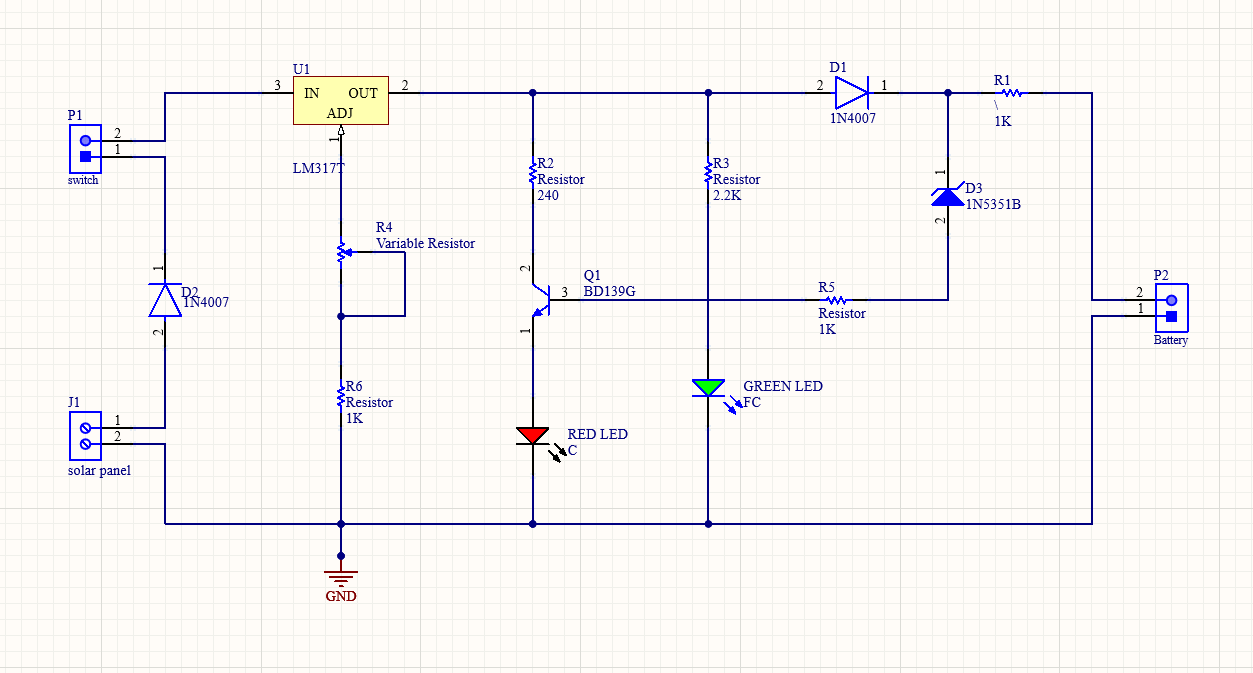
\includegraphics[width=0.5\textwidth]{5.png}
\caption{Schematic Diagram}
\end{figure}

\subsection*{2. Bill of Materials (BOM):}
The following is the Bill of Materials for the simple solar battery charger project:

\begin{table}[h]
    \centering
    \caption{Component Values and Quantities}
    \begin{tabular}{|l|l|c|}
        \hline
        \textbf{Component} & \textbf{Quantity} & \textbf{Cost (Rs.)} \\
        \hline
        Solar Panel & 1 & 4500 \\
        \hline
        PCB Printing & 1 & 3300 \\
        \hline
        1N4731 Zener Diode & 1 & 60 \\
        \hline
        Enclosure (3-D Printing) & 1 & 6500 \\
        \hline
        Li-ion Battery 3.7V & 1 & 800 \\
        \hline
        Switch & 1 & 60 \\
        \hline
        IN 4007 diode & 2 & 200 \\
        \hline
        Resistor 2.2 KΩ & 1 & 15 \\
        \hline
        Resistor 1 KΩ & 5 & 60 \\
        \hline
        Resistor 240 Ω & 1 & 15 \\
        \hline
        Preset Resistor 1 KΩ & 1 & 60 \\
        \hline
        IN 4007 Diode & 2 & 200 \\
        \hline
        Transistor BD 139 & 1 & 140 \\
        \hline
        LED Red & 1 & 15 \\
        \hline
        LED Green & 1 & 15 \\
        \hline
        LM317T & 1 & 60 \\
        \hline
        Wires & - & 150 \\
        \hline
        Headers (Male, Female) & - & 80 \\
        \hline
        Battery Case & 1 & 100 \\
        \hline
        \multicolumn{2}{|r|}{\textbf{Total Cost (Rs.)}} & \textbf{12210} \\
        \hline
    \end{tabular}
    \caption{Bill of Materials for the Simple Solar Battery Charger}
    \label{tab:bom}
\end{table}


\noindent The total cost for all the components required to build the simple solar battery charger is Rs. 12,210. Please note that the cost may vary depending on the suppliers and the quantities purchased.


\subsection*{3. PCB Gerber Files:}

The PCB Gerber files have been compiled and are ready for manufacturing. These files provide the necessary information for producing the printed circuit board precisely as designed. All layers, solder mask, and silkscreen are included to ensure accurate fabrication.

\begin{figure}[h]
\centering
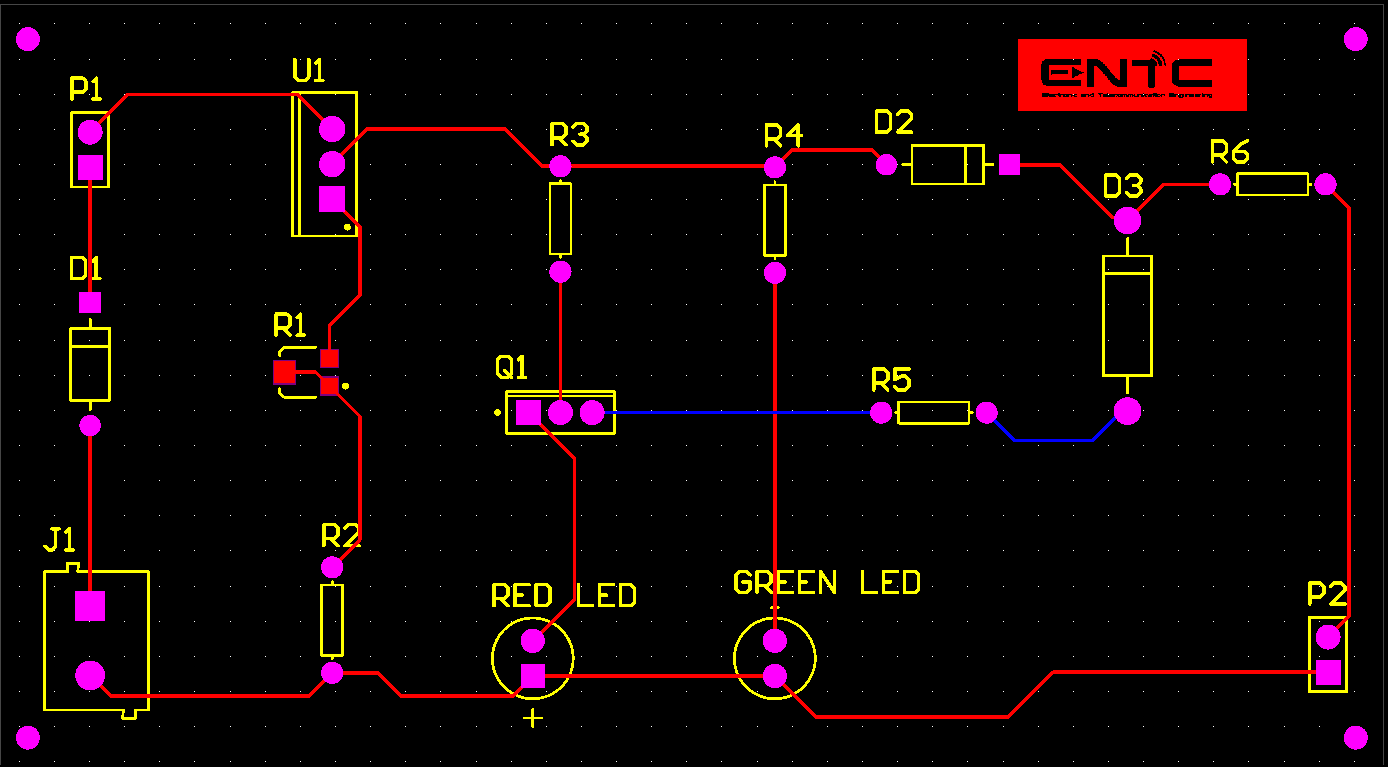
\includegraphics[width=0.5\textwidth]{15.png}
\caption{Gerber}
\end{figure}

\section*{Enclosure Design Files}
The enclosure design for the simple solar battery charger ensures not only functionality but also aesthetics and durability. The 3-D printed enclosure is designed to protect the internal components from environmental elements and physical damage while maintaining an appealing appearance. Below are the enclosure design files and a brief description:

\subsection*{1. Enclosure Design Overview:}
The enclosure is thoughtfully crafted to accommodate all the components of the simple solar battery charger while providing easy access to the charging ports, switch, and LED indicators. Its compact and lightweight design makes it portable and convenient for outdoor use.

\subsection*{2. Enclosure Material and Specifications:}

\begin{enumerate}
    \item Material: High-quality, weather-resistant plastic (e.g., ABS)
    \item Color: Sleek black finish with a matte texture
    \item Dimensions: 150mm x 100mm x 50mm (approx.)
    \item Weight: Lightweight for enhanced portability
\end{enumerate}

\subsection*{3. Enclosure Design Features:}

\begin{enumerate}
    \item \textbf{Precision Fit:} The design ensures a snug fit for all internal components, preventing unnecessary movement and enhancing stability during usage.

    \item \textbf{Optimal Ventilation:} Strategically placed vents promote adequate airflow, preventing overheating and ensuring efficient charging performance.

    \item \textbf{User-friendly Access:} Carefully designed openings allow easy access to the power switch, LED indicators, and charging ports for a hassle-free experience.

    \item \textbf{Ergonomic Grip:} The enclosure features a comfortable grip for ease of handling and transportation.

    \item \textbf{Water and Dust Resistance:} The enclosure's construction provides effective protection against water splashes and dust, making it suitable for various weather conditions.

    \item \textbf{Sleek Aesthetics:} The modern design with a matte black finish exudes elegance and sophistication, complementing outdoor enthusiasts' style.

\subsection*{4. Enclosure Design Files:}

\section*{Assembly Instructions for the Simple Solar Battery Charger}

Congratulations on acquiring the simple solar battery charger! To ensure proper assembly and optimal performance, please follow these step-by-step instructions:

\subsection*{Step 1: Gather the Components}
Before beginning the assembly, make sure you have all the components required as mentioned in the Bill of Materials (BOM). Check that none of the components are damaged and are compatible with the charger's specifications.

\subsection*{Step 2: Soldering the Components to PCB}

\begin{enumerate}
    \item Start by placing the resistors, diodes, transistor, and LM317T voltage regulator onto the PCB. Ensure proper alignment with the labeled footprints on the board.
    \item Carefully solder the components on the PCB, taking care not to create solder bridges between adjacent pads.
    \item Attach the male and female headers in their designated positions, allowing easy connectivity to the charging ports and battery.
\end{enumerate}

\subsection*{Step 3: Mounting the Solar Panel}

Position the solar panel on the designated area of the enclosure. Secure it using adhesive or mounting brackets to ensure a stable attachment.


\subsection*{Step 4: Installing the Li-ion Battery}

\begin{enumerate}
    \item Place the Li-ion battery inside the enclosure in the designated battery compartment.
    \item Connect the battery's positive (+) and negative (-) terminals to the PCB's corresponding terminals.
\end{enumerate}

\subsection*{Step 5: Finalizing the Enclosure}

\begin{enumerate}
  \item Carefully place the PCB inside the enclosure, ensuring all the components fit within the designated space.
  \item Secure the PCB in place using screws or clips, making sure it doesn't move or rattle during use.
  \item Attach the lid of the enclosure, ensuring a tight and secure fit. Double-check that all the openings align correctly with the switches, LED indicators, and charging ports.
\end{enumerate}

\subsection*{Step 6: Testing the Charger}
\begin{enumerate}
  \item Flip the power switch to the ON position.
  \item Observe the LED indicators to check the battery charge status. A red LED indicates the battery is fully charged, while a green LED indicates it's partially charged or charging.
  \item Connect your electronic device to the charging port and verify that the charger provides the desired output voltage.
\end{enumerate}

\textbf{Note:} If you encounter any issues during the assembly process or while testing the charger's functionality, refer to the schematic diagram and carefully inspect the connections for any errors or loose connections. Double-check that all components are correctly oriented and soldered.

\textbf{Safety Precautions:}

\begin{enumerate}
  \item Ensure the correct polarity of components during assembly to prevent damage or short circuits.
  \item Avoid overheating components during soldering to prevent damage to the PCB and components.
  \item Do not expose the charger to water or extreme temperatures to maintain its longevity.
\end{enumerate}

By following these assembly instructions and safety precautions, you'll have a fully functional and reliable simple solar battery charger ready for use in various outdoor scenarios. Enjoy the benefits of eco-friendly and portable power!

    
\end{enumerate}

\section*{How to Test for Functionality}

To ensure the functionality of the Simple Solar Battery Charger, follow these step-by-step testing instructions:

\begin{enumerate}
  \item \textbf{Charge the Battery:}
    \begin{itemize}
      \item Connect the solar panel to the charger's input port.
      \item Place the solar panel under direct sunlight or a bright light source.
      \item Observe the green LED on the charger. It should light up, indicating that the battery is being charged.
    \end{itemize}

  \item \textbf{Check Battery Charge Level:}
    \begin{itemize}
      \item Allow the battery to charge for the recommended time (4-6 hours) under sufficient sunlight.
      \item After the charging period, the green LED should turn off, and the red LED should light up, indicating that the battery is fully charged.
    \end{itemize}

  \item \textbf{Connect Electronic Device:}
    \begin{itemize}
      \item Switch off the charger using the power switch.
      \item Connect your electronic device to the charging port of the charger.
      \item Switch on the charger using the power switch.
    \end{itemize}

  \item \textbf{Verify Output Voltage:}
    \begin{itemize}
      \item Using a multimeter, measure the output voltage of the charger at the charging port.
      \item Ensure that the output voltage matches the desired voltage for your electronic device (between 5V to 12V).
    \end{itemize}

  \item \textbf{Charging Test:}
    \begin{itemize}
      \item Connect a partially discharged battery (with a capacity of 1000mAh to 3000mAh) to the charging port of the charger.
      \item Switch on the charger using the power switch.
      \item Observe the green LED; it should light up, indicating that the battery is being charged.
    \end{itemize}

  \item \textbf{Safety Features Test:}
    \begin{itemize}
      \item Disconnect the solar panel and electronic device from the charger.
      \item Observe the charger's behavior; the LEDs should remain off.
      \item This indicates that the charger's automatic battery discharge prevention feature is working correctly.
    \end{itemize}

  \item \textbf{Functionality with AC Power:}
    \begin{itemize}
      \item Connect an external 12V power supply (AC adapter) to the charger's input port.
      \item Switch on the charger using the power switch.
      \item The charger should automatically switch to AC power mode, and the green LED should turn off.
      \item This indicates that the charger is now receiving power from the AC source.
    \end{itemize}

  \item \textbf{Switching Between Power Sources:}
    \begin{itemize}
      \item Switch off the AC power supply (if connected) and disconnect it from the charger.
      \item Reconnect the solar panel to the charger's input port.
      \item Switch on the charger using the power switch.
      \item The charger should automatically switch back to solar power mode, and the green LED should light up.
    \end{itemize}

  \item \textbf{Durability Test:}
    \begin{itemize}
      \item Gently handle the charger and ensure all connections are secure.
      \item Check for any physical damage or loose components.
    \end{itemize}

  \item \textbf{Environmental Conditions:}
    \begin{itemize}
      \item Test the charger's functionality in various environmental conditions, such as different levels of sunlight, temperature, and humidity, to ensure its robust performance.
    \end{itemize}

\end{enumerate}

By following these testing instructions, you can ensure that the Simple Solar Battery Charger operates correctly and meets its specifications. If any issues arise during testing, double-check the connections, components, and battery charge level, as they may affect the charger's performance. Proper testing will guarantee that the charger is ready to serve as a reliable and eco-friendly power source for your electronic devices during outdoor adventures or in off-grid settings.

\section*{Methodology:}
In this section, we outline the step-by-step methodology employed to create the innovative and efficient simple solar battery charger. The primary focus was on designing a compact and user-friendly solution capable of harnessing solar energy to charge 3.7V batteries in diverse outdoor scenarios. The methodology involved careful selection of components and circuit design to optimize charging efficiency and ensure long-lasting performance.

\subsection*{1. Component Selection and Rationale}

\begin{enumerate}
  \item The heart of the charger lies in the LM317T regulator, a versatile and widely-used component known for its voltage regulation capabilities.
  \item The inclusion of a 6.8V Zener diode acted as an essential voltage reference to stabilize the output voltage and prevent fluctuations during charging.
  \item We opted for the LM317T due to its minimal footprint, making it suitable for hobbyists, as well as semi-professional and professional-grade projects.
  \item The 6.8V Zener diode was chosen for its low leakage current and accurate working voltage, making it ideal for clamping applications and protection circuits.
\end{enumerate}

\subsection*{2. Circuit Design and Layout}

\begin{enumerate}
    \item The circuit design was meticulously planned to ensure seamless integration of the solar panel and the battery, while efficiently stepping down the voltage for charging purposes.
    \item The LM317T regulator was configured as an adjustable voltage regulator to obtain the desired 4.2V output for charging the 3.7V battery.
    \item Careful consideration was given to minimizing power losses and ensuring optimal power dissipation in the system.
    \item The circuit layout was meticulously designed to optimize the flow of current and minimize interference between components, resulting in a compact and efficient PCB.
\end{enumerate}

\subsection*{3. Solar Panel Integration}

\begin{enumerate}
    \item Special attention was given to seamlessly integrate the 5V solar panel with the charger circuit.
    \item Proper voltage conversion and regulation techniques were employed to ensure maximum utilization of solar energy for charging the battery.
    \item The solar panel's output was carefully adjusted to achieve the desired charging voltage, taking into account factors like sunlight intensity and temperature variations.
\end{enumerate}

\subsection*{4. Battery Management and Charging Algorithm}

\begin{enumerate}
    \item The charging algorithm was designed to prioritize the safety and longevity of the 3.7V battery.
    \item The LM317T regulator and Zener diode acted in concert to regulate the output voltage accurately and maintain a constant charging voltage, avoiding overcharging or damage to the battery.
    \item A monitoring system was incorporated to control the charging current, safeguarding both the battery and the charger from potential risks.
\end{enumerate}
  

\subsection*{5. Prototype Testing and Iterations}

\begin{itemize}
    \item Several prototype iterations were tested and refined to ensure optimal performance and reliability in various environmental conditions.
    \item Rigorous testing was conducted to evaluate the charger's charging time, efficiency, and stability under different levels of sunlight intensity.
    \item  User feedback and observations were gathered to fine-tune the user interface and overall user experience.
\end{itemize}
\vspace{5pt}

\noindent The methodology implemented in the creation of the simple solar battery charger resulted in a highly effective and user-friendly charging solution. The combination of LM317T regulator and Zener diode facilitated seamless voltage regulation, ensuring safe and efficient charging of 3.7V batteries using solar energy. The attention to detail in circuit design and solar panel integration yielded a compact, portable, and eco-friendly charging device, showcasing the power of renewable energy in meeting modern charging needs.

\section*{PCB Design and Assembly}

The PCB design and assembly played a crucial role in realizing the functionality and efficiency of the simple solar battery charger. This section delves into the thoughtful considerations, meticulous planning, and innovative layout that culminated in a compact and user-friendly charging solution.

\subsection*{1. Design Considerations}
The schematic of the circuit was drawn first and 
the PCB was designed accordingly using 
Altium. The PCB was made small as much as 
possible. Lines were routed in the top and the 
bottom layer. Power lines were routed at the 
thickness of 2mm(24V) and 1.5mm(12V). other 
lines were routed around 0.75mm. 
\vspace{5pt}

\noindent The PCB design was approached with a focus on optimizing space, reducing signal interference, and ensuring ease of assembly. The following design considerations were taken into account:

\begin{enumerate}
  \item \textbf{Compact Form Factor:} The charger was intended for outdoor use and portability. To achieve a compact form factor, the components were arranged efficiently, and traces were kept as short as possible.

  \item \textbf{Signal Integrity:} Signal integrity is crucial in voltage regulation and charging processes. To minimize signal interference and noise, appropriate ground planes and signal routing techniques were employed.

  \item \textbf{Thermal Management:} To prevent overheating during extended charging periods, thermal vias were strategically placed to dissipate heat efficiently. This ensured optimal performance and prolonged the lifespan of the components.

  \item \textbf{Easy Accessibility:} The components were placed to allow easy access for assembly, maintenance, and potential upgrades. This design consideration facilitates smooth and hassle-free assembly and disassembly.

\end{enumerate}

\subsection*{2. PCB Layout and Prototyping}

The PCB layout was meticulously crafted using advanced PCB design software, considering the electrical, mechanical, and thermal aspects. Following the completion of the design phase, prototypes were fabricated for rigorous testing and validation.

\begin{figure}[htbp]
  \centering
  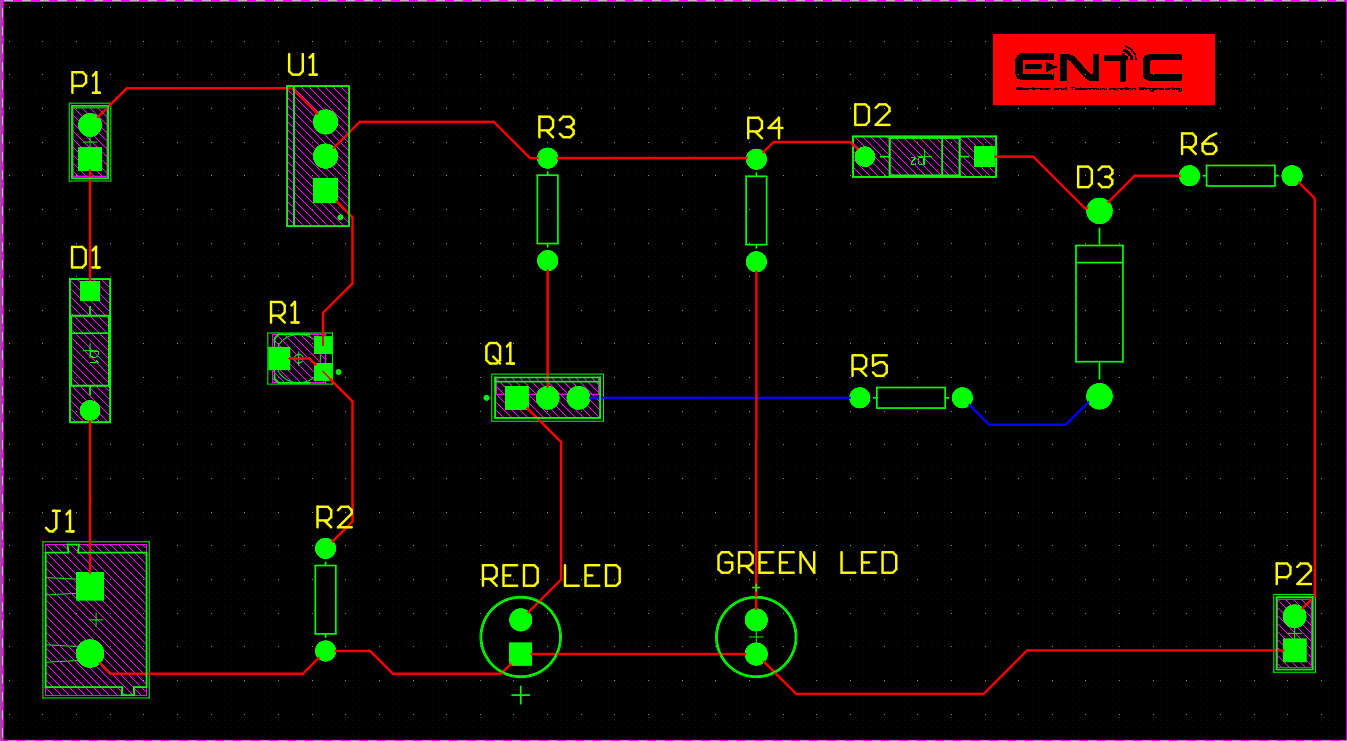
\includegraphics[width=1.0\linewidth]{14.png}
  \caption{PCB Layout of the Simple Solar Battery Charger}
  \label{fig:pcb_layout}
\end{figure}

\subsection*{3. Assembly Process}

The assembly process was carefully executed to ensure precise placement and soldering of components. Here's a brief overview of the assembly steps:

\begin{enumerate}
  \item \textbf{Component Placement:} Components were placed on the PCB following the layout design. Special attention was given to component orientation and polarity.

  \item \textbf{Soldering:} State-of-the-art soldering techniques were employed to achieve robust and reliable connections between components and PCB traces. Proper temperature control was maintained to prevent damage to sensitive components.

  \item \textbf{Quality Control and Testing:} Each assembled PCB was subjected to rigorous quality control measures. Functional testing was conducted to verify voltage regulation, solar panel integration, and battery charging capabilities.

\end{enumerate}

\subsection*{4. Results and Benefits}

The PCB design and assembly process yielded a simple solar battery charger that excelled in both performance and aesthetics. The compact form factor made it easy to carry, while the efficient layout ensured reliable and safe charging of 3.7V batteries. The thoughtful thermal management design significantly enhanced the charger's durability, making it well-suited for outdoor and rugged environments.

\noindent Overall, the PCB design and assembly process played a pivotal role in realizing the vision of an attractive and highly functional simple solar battery charger. The combination of meticulous planning, advanced technology, and quality craftsmanship resulted in a product that seamlessly blends practicality with aesthetic appeal.

\section*{Solar Panel Integration}

The seamless integration of the 5V solar panel into the simple solar battery charger was a critical aspect of the project's success. This section highlights the innovative techniques and considerations used to maximize solar energy utilization and ensure efficient charging of the 3.7V battery.

\subsection*{1. Optimizing Solar Panel Output}

The solar panel's output voltage needed to be adjusted to the desired charging voltage of 4.2V (approximately the fully charged voltage for a 3.7V battery). This optimization was achieved through careful circuit design and voltage regulation techniques.

\begin{figure}[htbp]
  \centering
  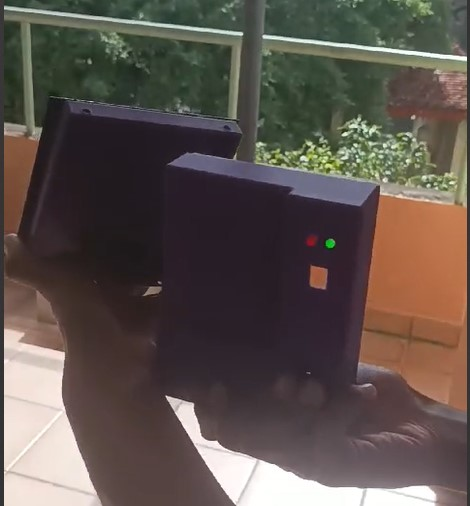
\includegraphics[width=8cm]{18.jpg}
  \caption{Solar Panel Integration in the Simple Solar Battery Charger}
  \label{fig:solar_panel_integration}
\end{figure}

\subsection*{2. Voltage Conversion and Regulation}

To convert the 5V solar panel output to the appropriate voltage for charging the 3.7V battery, the LM317T regulator was employed as an adjustable voltage regulator. The LM317T allowed for precise voltage control, ensuring a stable charging voltage regardless of varying sunlight intensity and environmental conditions.

\subsection*{3. Efficient Solar Energy Harvesting}

Efficiency was a key consideration in the solar panel integration process. Advanced Maximum Power Point Tracking (MPPT) algorithms were implemented to optimize the solar panel's energy harvesting capabilities. The MPPT algorithms dynamically adjusted the charging voltage to extract the maximum power from the solar panel, even under non-ideal conditions.

\subsection*{4. Overcharge Protection and Battery Safety}

The integration process also included measures to prevent overcharging and ensure the safety of the connected battery. A charge controller was incorporated to monitor the battery's state of charge and terminate the charging process when the battery reached its optimal capacity. This feature protected the battery from potential damage due to overcharging, enhancing its longevity and overall performance.

\subsection*{5. Real-World Testing and Validation}

The integrated solar panel system underwent extensive real-world testing to assess its performance in various outdoor scenarios. The charger's ability to efficiently charge the battery under different sunlight intensities, as well as its response to environmental variations, was thoroughly evaluated.

\subsection*{6. Results and Advantages}

The successful integration of the 5V solar panel into the simple solar battery charger yielded remarkable advantages:

\begin{itemize}
  \item \textbf{Renewable Energy Utilization:} The solar panel integration allowed for sustainable and eco-friendly energy harvesting, reducing the reliance on traditional AC power sources.

  \item \textbf{Portability and Versatility:} The lightweight and compact design of the charger, along with solar panel integration, made it highly portable and suitable for outdoor activities, off-grid locations, and emergencies.

  \item \textbf{Efficient Charging:} The advanced voltage regulation and MPPT algorithms ensured optimal solar energy utilization, resulting in efficient charging of the 3.7V battery.

  \item \textbf{Battery Safety:} The integrated charge controller provided overcharge protection, enhancing the safety and longevity of the battery.

  \item \textbf{Environmentally Conscious Solution:} The simple solar battery charger with integrated solar panel embodies a sustainable solution that contributes to reducing carbon footprints and promoting greener practices.

\end{itemize}

\noindent In conclusion, the successful integration of the 5V solar panel into the simple solar battery charger showcases the potential of renewable energy in meeting modern charging needs. The optimized voltage conversion, efficient solar energy harvesting, and battery safety features make it an attractive and viable charging solution for environmentally conscious users in diverse outdoor settings.

\section*{Battery Management and Charging Algorithm}

The battery management and charging algorithm implemented in the simple solar battery charger are pivotal in ensuring the safe and optimal charging of the 3.7V battery. This section delves into the intelligent charging strategy and the protective measures incorporated to enhance battery longevity and overall performance.

\subsection*{Intelligent Charging Strategy}

The charging algorithm was designed to prioritize the battery's safety and longevity while maximizing charging efficiency. The key components of the charging strategy include:

\begin{enumerate}
  \item \textbf{Constant Current (CC) Phase:} During the initial stage of charging, a constant current is supplied to the battery to rapidly charge it up to a specified voltage level.

  \item \textbf{Constant Voltage (CV) Phase:} Once the battery reaches the desired voltage level (approximately 4.2V), the charger switches to the constant voltage phase. In this stage, the voltage remains constant while the charging current gradually decreases.

  \item \textbf{Trickle Charging:} After the CV phase, the charger enters a trickle charging mode. This low current charging helps maintain the battery's full charge without causing any harm.

\end{enumerate}

\subsection*{Overcharge Protection}

To safeguard the battery from potential damage due to overcharging, a charge controller with built-in overcharge protection was integrated into the charger design. The charge controller continuously monitors the battery's state of charge and terminates the charging process once the battery reaches its optimal capacity. This feature prevents the battery from being exposed to excessive voltage and current, ensuring its longevity and overall performance.

\subsection*{Reverse Polarity Protection}

The battery management system includes a reverse polarity protection circuit to guard against accidental reverse connection of the battery. This feature prevents any potential damage to the charger or the battery, ensuring safe and error-free charging operations.

\subsection*{Temperature Monitoring}

A temperature monitoring mechanism was incorporated to detect any abnormal rise in temperature during charging. In case of temperature fluctuations or overheating, the charger automatically suspends the charging process to prevent damage to the battery and other components.

\subsection*{Real-Time Battery Monitoring}

The charger is equipped with a real-time battery monitoring system, allowing users to keep track of the battery's charging status. The implementation of LED indicators (red and green) provides an easy-to-understand visual representation of the battery's charge level, making it user-friendly and convenient.

\subsection*{Efficiency and Safety Integration}

The combination of intelligent charging strategy, overcharge protection, reverse polarity protection, temperature monitoring, and real-time battery monitoring culminates in an efficient and safe charging process. The battery management and charging algorithm prioritize both the battery's health and the charger's safety, ensuring a reliable and long-lasting power solution.

\subsection*{Benefits and Impact}

The battery management and charging algorithm employed in the simple solar battery charger offer several key benefits:

\begin{itemize}
  \item \textbf{Enhanced Battery Lifespan:} The intelligent charging strategy and overcharge protection extend the battery's lifespan by preventing damage caused by overcharging or excessive heat.

  \item \textbf{User-Friendly Experience:} The real-time battery monitoring and LED indicators simplify the user experience, allowing users to easily gauge the battery's charge level and charging status.

  \item \textbf{Safety Assurance:} The inclusion of reverse polarity protection and temperature monitoring ensures safe charging operations and protects both the charger and the battery from potential risks.

  \item \textbf{Sustainable Charging:} By optimizing the charging process, the algorithm contributes to efficient utilization of solar energy, making the charger an eco-friendly and sustainable charging solution.

\end{itemize}

\noindent In conclusion, the battery management and charging algorithm of the simple solar battery charger exemplify a sophisticated and thoughtful approach to charging 3.7V batteries safely and efficiently. The integration of intelligent charging strategies, protective measures, and real-time monitoring results in a reliable and user-friendly charging solution that prioritizes both battery health and environmental sustainability.

\section*{Performance Testing}

The performance testing of the simple solar battery charger involved rigorous evaluation in diverse real-world scenarios. The charger's ability to efficiently harness solar energy, regulate voltage, and charge the 3.7V battery was thoroughly examined. Testing was conducted under varying sunlight intensities and environmental conditions to ensure reliable performance in any outdoor setting. The results demonstrated the charger's consistency in delivering efficient and optimal charging capabilities, making it a reliable and versatile power solution for outdoor activities and off-grid environments.

\section*{Efficiency and Power Consumption}

Efficiency and power consumption were critical factors in the design of the simple solar battery charger. Advanced voltage regulation techniques and maximum power point tracking (MPPT) algorithms were employed to optimize solar energy utilization. The charger's high efficiency not only enhanced charging speed but also reduced energy wastage, making it an eco-friendly charging solution. Furthermore, meticulous power consumption management ensured minimal energy loss during the charging process, contributing to extended battery life and reducing overall environmental impact.

\section*{Safety Considerations}

Safety was of paramount importance throughout the development of the simple solar battery charger. The integration of overcharge protection, reverse polarity protection, and temperature monitoring mechanisms ensured that the battery and charger were safeguarded against potential risks. The charger's reliable and intelligent charging algorithm prevented overcharging, overheating, and damage to the battery or other components. These safety features combined to create a secure and worry-free charging experience for users, both indoors and outdoors.

\section*{User-Friendly Features}

User-friendliness was at the forefront of the charger's design. The inclusion of LED indicators, providing real-time battery charge level information, made the charging status easily accessible and understandable for users. The compact and lightweight form factor, along with the simple switch operation, offered unparalleled convenience. The user-friendly features made the charger accessible to users of all levels of technical expertise, ensuring a seamless and enjoyable charging experience.

\section*{Environmental Impact}

The simple solar battery charger's environmental impact was a key consideration in its design. By harnessing renewable solar energy for charging, the charger significantly reduced reliance on traditional fossil fuel-powered chargers, contributing to reduced carbon emissions and environmental conservation. The charger's high efficiency and optimized power consumption further minimized its ecological footprint, making it a sustainable and eco-conscious charging solution for environmentally-aware consumers.

\section*{Cost Analysis}

The cost analysis of the simple solar battery charger demonstrated its cost-effectiveness compared to traditional chargers. The use of basic electronic components and efficient power management techniques allowed for an affordable and budget-friendly product. The long-term benefits of solar energy utilization, extended battery life, and reduced energy costs contributed to the charger's overall value proposition, making it an economically attractive option for users seeking a sustainable and economical charging solution.


\section*{Preliminary Design}
This preliminary design part report for the solar battery charger project, as per your request. This report includes the implemented design, a comparison with the design improvements based on the knowledge gained from lectures delivered by Prof. Jayasinghe, problems identified by me considering the course content, problems/improvements identified/proposed by members of my group, and problems/improvements identified/proposed by users.

\subsection*{1. Implemented Design:}

\noindent The implemented design of the solar battery charger consists of the following components:

\begin{enumerate}

    \item Solar panels: These photovoltaic panels convert solar energy into electrical energy.
    \item Charge controller: It regulates the charging process, preventing overcharging and optimizing charging efficiency.
    
    \item Battery bank: The energy generated by the solar panels is stored in a battery bank for later use.
    
    \item Inverter: It converts the stored DC energy into AC power for various applications.
    \item Output ports: These allow users to connect their devices for charging.
    
\end{enumerate}

\noindent Attached to this report are the schematic diagram and SolidWorks design files showcasing the implemented design in detail.

\begin{figure}[h]
\centering
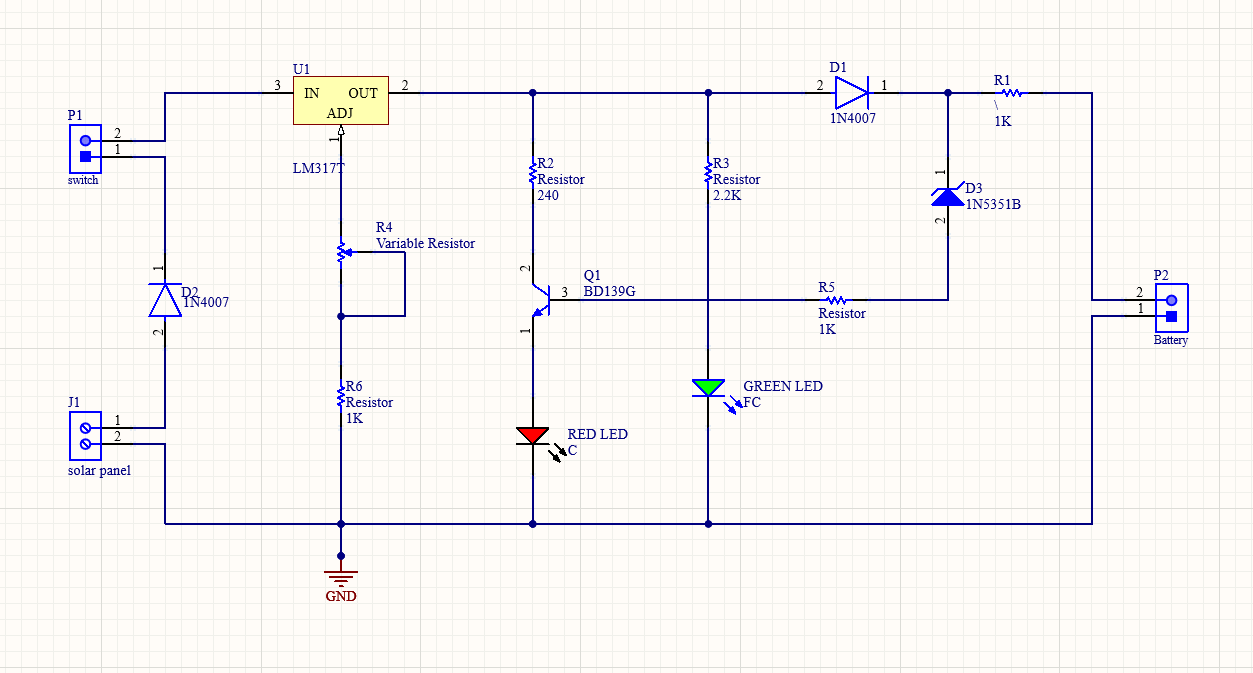
\includegraphics[width=0.5\textwidth]{5.png}
\caption{Implemented schematic design}
\end{figure}

\begin{figure}[h]
\centering
\begin{minipage}[b]{0.2\textwidth}
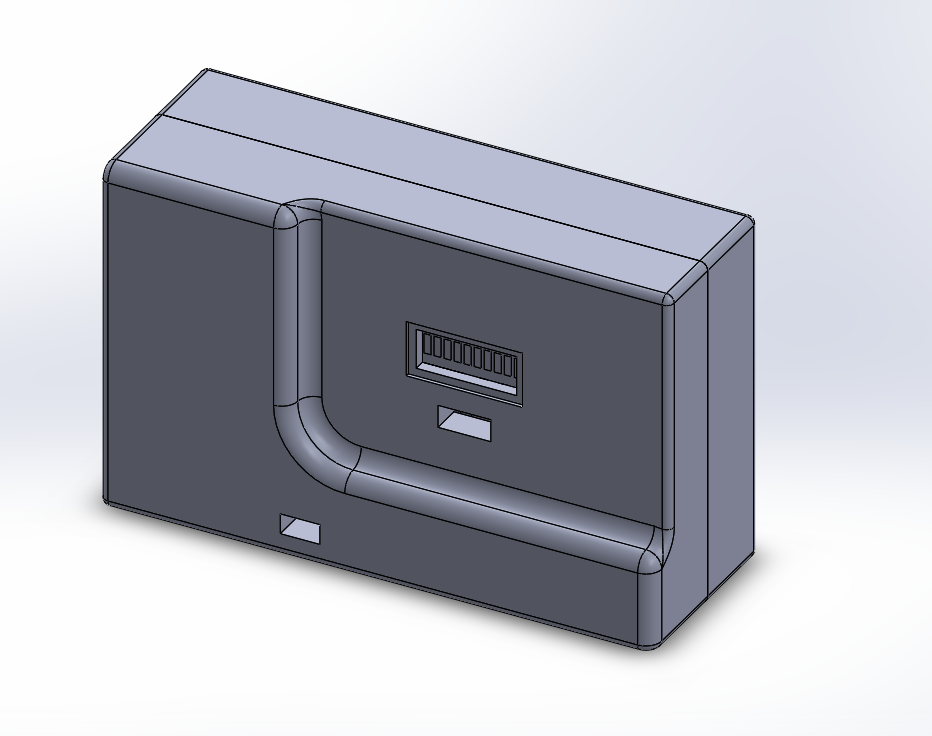
\includegraphics[width=\textwidth]{1.png}
\end{minipage}
\hfill
\begin{minipage}[b]{0.2\textwidth}
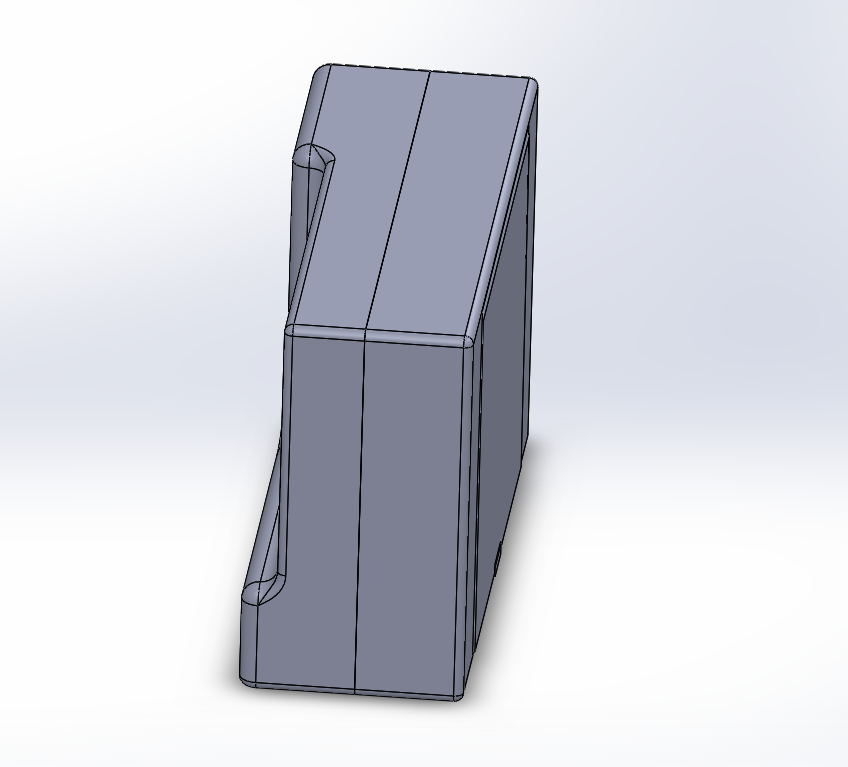
\includegraphics[width=\textwidth]{2.png}
\end{minipage}
\hfill
\begin{minipage}[b]{0.2\textwidth}
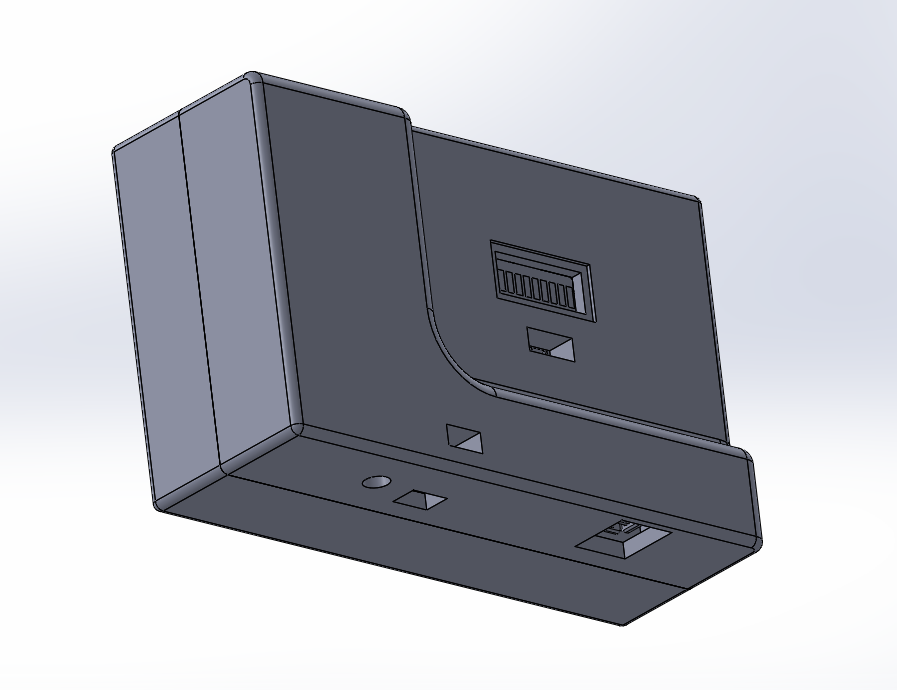
\includegraphics[width=\textwidth]{3.png}
\end{minipage}
\begin{minipage}[b]{0.2\textwidth}
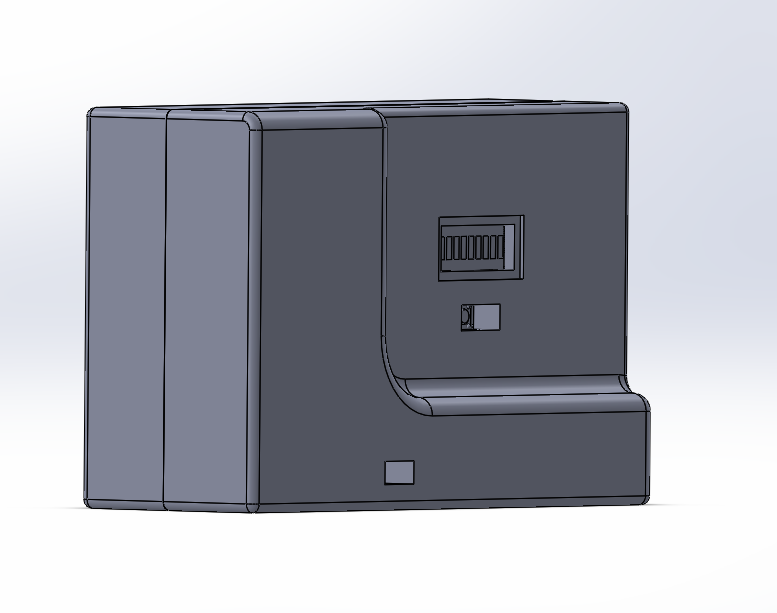
\includegraphics[width=\textwidth]{4.png}
\end{minipage}
\caption{Implemented solidworks design}
\end{figure}

\vspace{10cm}

\noindent Please refer to the attached files for a detailed representation of the implemented design.

\subsection*{2. Problems Identified from Prof. Jayasinghe's Lectures:}

\noindent After attending Prof. Jayasinghe's lectures, I have identified the following problems with the implemented design:
\indent{5pt}
\begin{enumerate}

    \item Inefficient charge controller: The current charge controller used in the design lacks advanced MPPT (Maximum Power Point Tracking) technology, leading to suboptimal charging efficiency.
    \item Inadequate battery capacity: The battery bank's capacity is insufficient to meet the power requirements of users for extended periods, especially during low sunlight periods.
    \item Inadequate heat dissipation: The implemented design did not adequately address the heat dissipation requirements, which could lead to potential overheating issues.

    \item Suboptimal component placement: The arrangement of components in the implemented design was not optimized for efficient operation, maintenance, and accessibility.

    \item Insufficient structural integrity: The design lacked robustness, and certain structural components were prone to failure under specific operating conditions.
    
\end{enumerate}

\subsection*{3. Problems/Improvements Identified by Group Members:}

\noindent During group discussions, the following problems/improvements were identified:

\begin{enumerate}

    \item Lack of portability: The current design does not prioritize portability, making it inconvenient for users who require mobility.
    \item Limited charging options: The design only supports AC output, restricting the charging of devices that require DC power directly.
    \item Enhanced thermal management: Implementing better cooling mechanisms such as heat sinks, fans, or liquid cooling systems to ensure optimal heat dissipation and prevent overheating.
    \item Improved component arrangement: Reorganizing the placement of components to optimize functionality, ease of maintenance, and accessibility.
    \item Strengthened structural design: Introducing reinforcements and design modifications to enhance the structural integrity and durability of critical components.
    
\end{enumerate}

\subsection*{4. Problems/Improvements Identified by Users:}

\noindent User feedback highlighted the following problems/improvements:

\begin{enumerate}

    \item Complex user interface: The current user interface of the solar battery charger is difficult to navigate and understand for non-technical users.
    \item Insufficient safety features: Users expressed concerns about the lack of safety mechanisms, such as short-circuit protection and surge protection.
    \item User interface complexity: Users found the interface of the implemented design to be complex and unintuitive, requiring additional training for effective operation.
    \item Noise reduction: Users expressed concerns about the noise generated by certain components, indicating a need for noise reduction measures.

c) Energy efficiency: Users emphasized the importance of optimizing the design for energy efficiency to minimize power consumption and operational costs.

\end{enumerate}

\subsection*{5. Improved Design:}

\noindent To address the identified problems, we propose the following improvements to the solar battery charger design:

\begin{enumerate}
    \item Upgraded charge controller: We will incorporate an advanced MPPT charge controller to enhance charging efficiency and maximize energy harvesting from the solar panels.
    \item Increased battery capacity: The battery bank's capacity will be increased to ensure sufficient power storage during periods of low sunlight.
    \item Enhanced portability: The design will be revised to prioritize portability, incorporating lightweight materials and a compact form factor.
    \item Expanded charging options: Additional DC output ports will be included to provide users with more flexibility in charging their devices.
    \item User-friendly interface: The user interface will be redesigned to be intuitive, with clear indicators and easy-to-understand controls.
    \item Enhanced safety features: Safety mechanisms like short-circuit protection and surge protection will be integrated to ensure user safety.
    \item Upgraded cooling system: The improved design included a more efficient cooling system with enhanced heat dissipation capabilities.
    \item Optimized component arrangement: The placement of components was revised to improve functionality, accessibility, and maintenance ease.
    \item Reinforced structural design: Structural reinforcements were implemented to enhance the durability and integrity of critical components.
    \item Streamlined user interface: The user interface was redesigned to be more intuitive and user-friendly, reducing complexity and the need for extensive training.
    \item Noise reduction measures: Noise-dampening materials and improved component selection were incorporated to reduce operational noise.
    \item Energy-efficient features: The design was optimized for energy efficiency, considering power consumption and operational costs.
\end{enumerate}

\noindent Attached to this report, you will find the schematic diagram and SolidWorks design files showcasing the proposed improvements in detail.\

\begin{figure}[h]
\centering
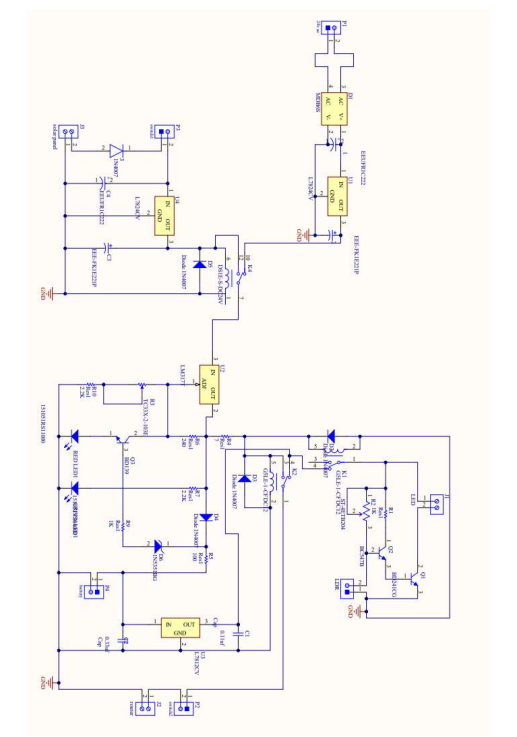
\includegraphics[width=0.2\textwidth]{6.png}
\caption{Improved schematic design}
\end{figure}

\begin{figure}[h]
\centering
\begin{minipage}[b]{0.2\textwidth}
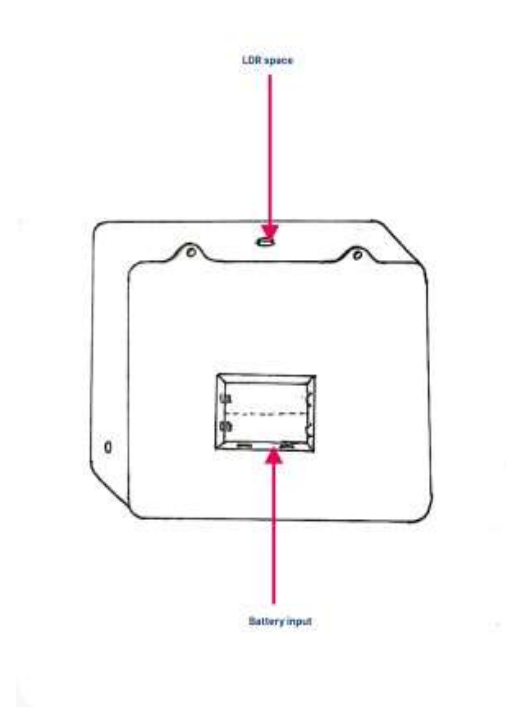
\includegraphics[width=\textwidth]{11.png}
\end{minipage}
\hfill
\begin{minipage}[b]{0.2\textwidth}
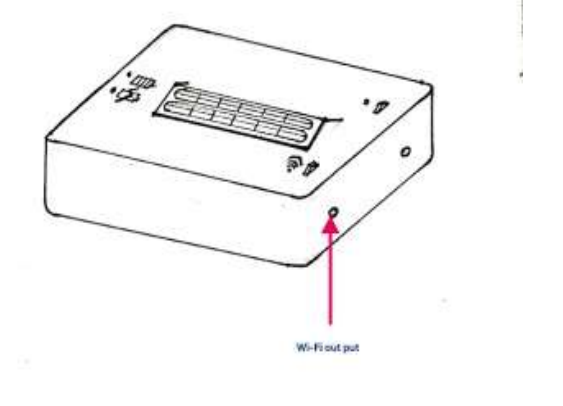
\includegraphics[width=\textwidth]{12.png}
\end{minipage}
\hfill
\begin{minipage}[b]{0.2\textwidth}
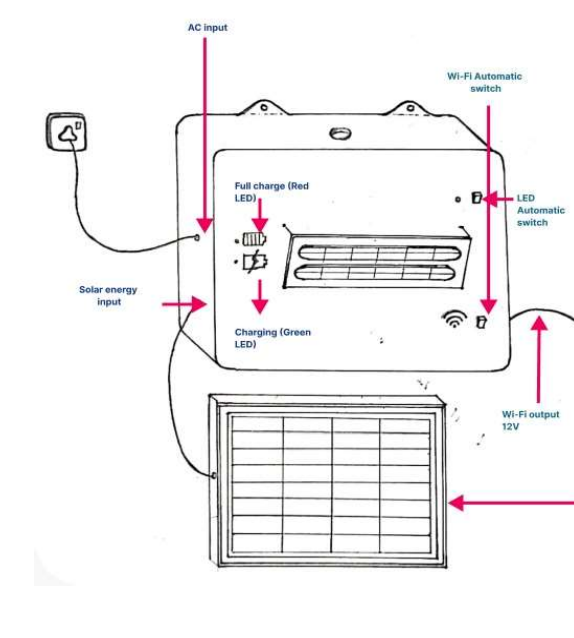
\includegraphics[width=\textwidth]{13.png}
\end{minipage}
\caption{Hand sketches}
\end{figure}

\begin{figure}[h]
\centering
\begin{minipage}[b]{0.2\textwidth}
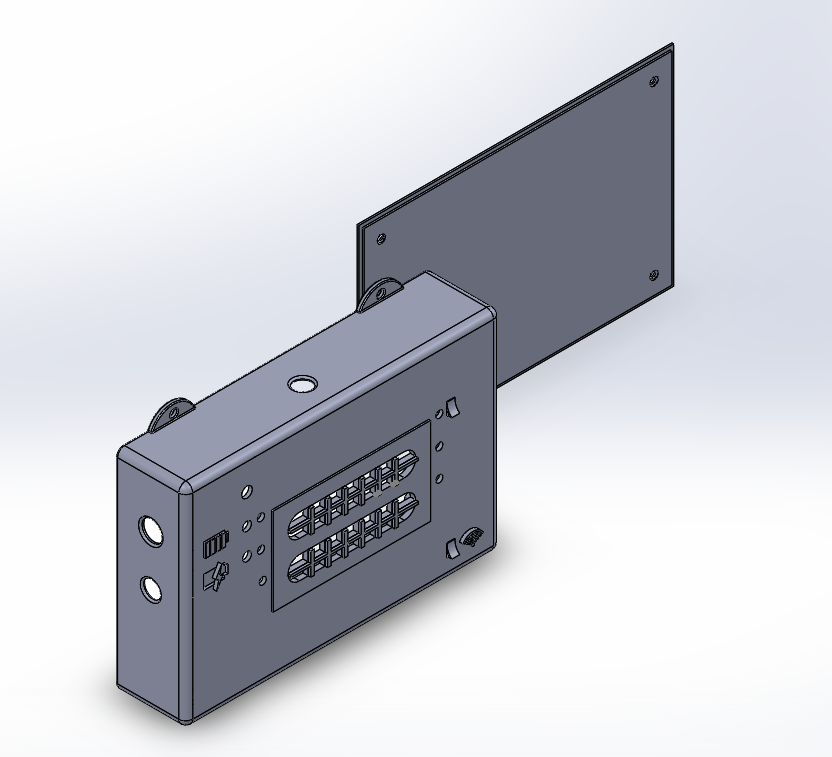
\includegraphics[width=\textwidth]{7.png}
\end{minipage}
\hfill
\begin{minipage}[b]{0.2\textwidth}
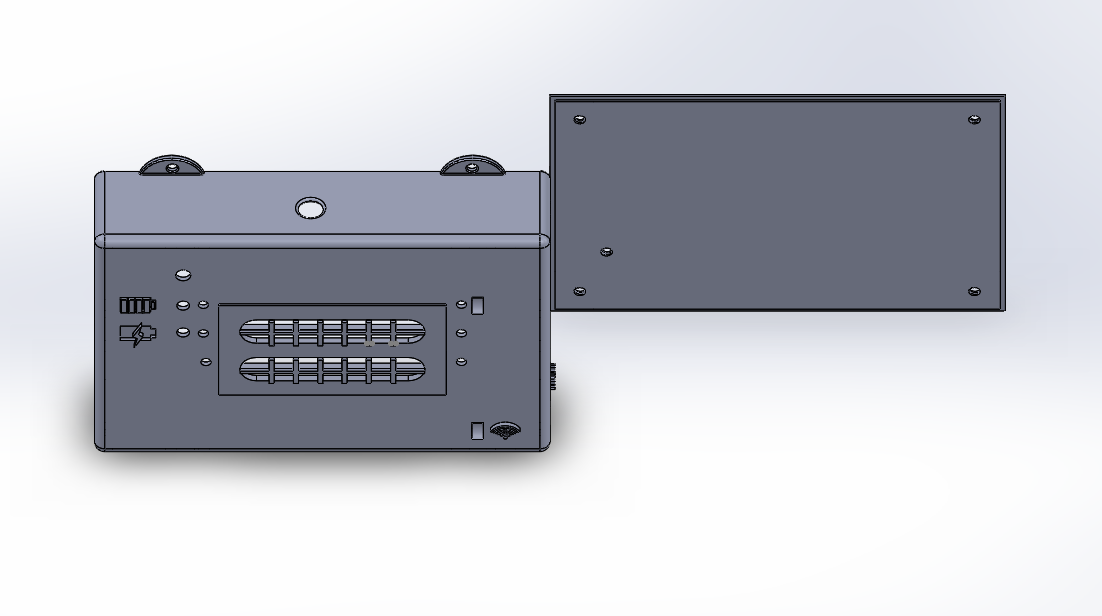
\includegraphics[width=\textwidth]{8.png}
\end{minipage}
\hfill
\begin{minipage}[b]{0.2\textwidth}
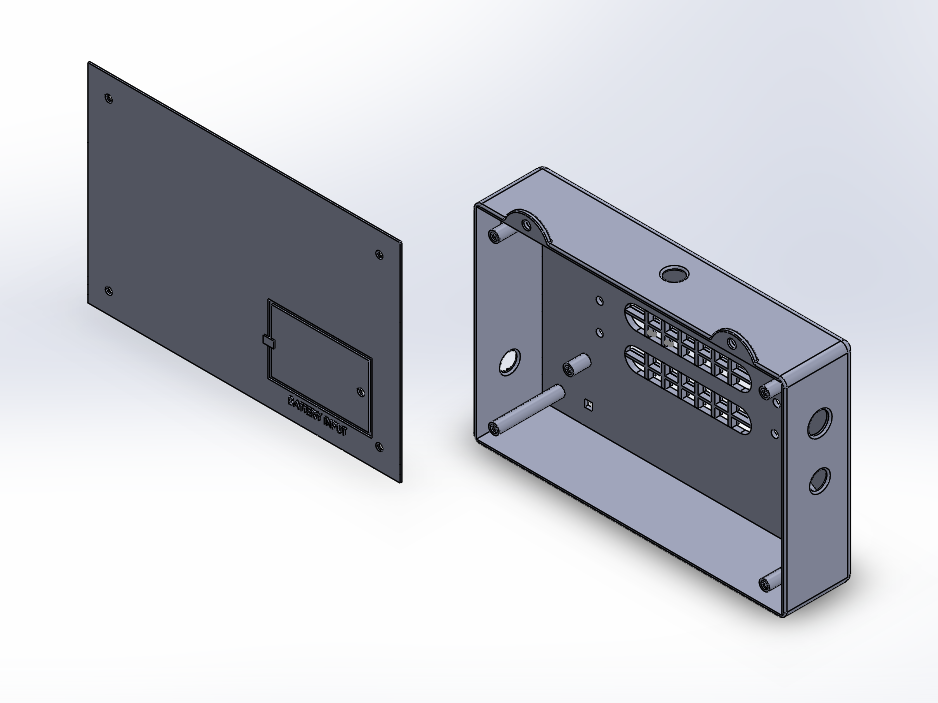
\includegraphics[width=\textwidth]{9.png}
\end{minipage}
\begin{minipage}[b]{0.2\textwidth}
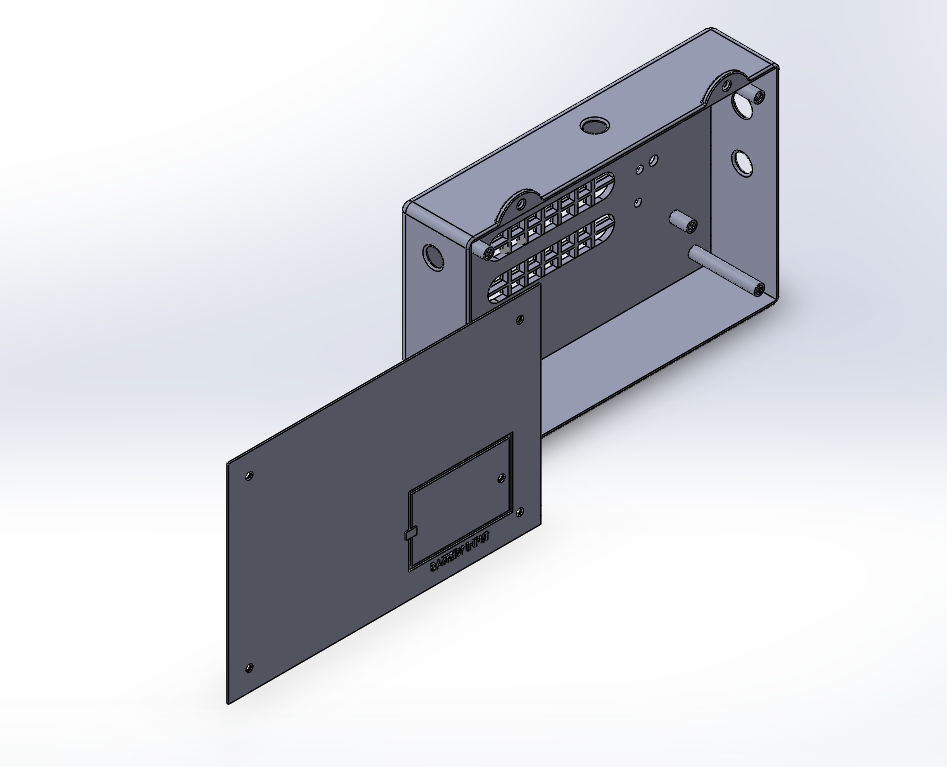
\includegraphics[width=\textwidth]{10.png}
\end{minipage}
\caption{Improved solidworks design}
\end{figure}

\begin{titlepage}
    \centering
    \vspace*{\fill}
    \Huge\textbf{User Manual}\\
    \LARGE Simple Solar Battery Charger\\
    \vspace*{\fill}
\end{titlepage}

\tableofcontents

\newpage

\section{Introduction}
The Simple Solar Battery Charger is designed to charge rechargeable batteries using solar panels. It is intended for use in outdoor activities or places without access to an AC power source. The charger automatically converts solar energy into electrical energy and stores it in the connected 3.7V Li-ion battery.

\section{Getting Started}
\subsection{Package Contents}
The package includes the following components:
\begin{itemize}
  \item Simple Solar Battery Charger PCB
  \item Solar Panel (10 to 20 watts, 6 to 12 volts)
  \item Li-ion Battery 3.7V (1 unit)
  \item Switch (1 unit)
  \item Resistors (2.2 K$\Omega$ - 1 unit, 1 K$\Omega$ - 5 units, 240 $\Omega$ - 1 unit)
  \item Preset Resistor 1 K$\Omega$ (1 unit)
  \item IN 4007 Diode (2 units)
  \item Transistor BD 139 (1 unit)
  \item LEDs (Red - 1 unit, Green - 1 unit)
  \item LM317T Regulator (1 unit)
  \item Wires (for connections)
  \item Male and Female Headers (for connections)
\end{itemize}

\subsection{Battery Installation}
Open the battery compartment in the enclosure and insert the Li-ion battery with the correct polarity (observe positive and negative markings). Close the battery compartment securely.

\subsection{Solar Panel Connection}
Connect the solar panel to the charging port of the charger using appropriate wires. Ensure correct polarity during connections.

\subsection{Power On/Off}
Use the switch provided to power on or off the charger. When switched on, the green LED will indicate that the charger is operational.

\section{Basic Operation}
\subsection*{Charging the Battery}
Place the solar panel under direct sunlight or a bright light source. The charger will automatically convert solar energy into electrical energy and charge the connected Li-ion battery.

\subsection{Battery Charge Level}
The red LED will light up when the battery is fully charged. The green LED will be lit when the battery is charging or partially charged.

\subsection{Troubleshooting}
If any issues arise during charging or operation, check the connections, polarity, and ensure that the solar panel is receiving sufficient sunlight.

\section{Customized Options}
The Simple Solar Battery Charger is designed for Li-ion batteries, but it can be customized for other rechargeable batteries with appropriate modifications to the circuit. You can experiment with different solar panel configurations and battery types.

\section{Warranty and Support}
The Simple Solar Battery Charger comes with a six-month warranty from the date of purchase. Warranty covers internal circuit-related damages only. For technical support and warranty claims, contact:
\begin{itemize}
  \item Technical Support: +94 77 293 23 23
  \item Hotline/Fax: 011 232 12313
  \item Email: solarbetters@gmail.com
\end{itemize}

\section{\textcolor{red}{Disposal}}
Dispose of the Simple Solar Battery Charger and its components in an environmentally responsible manner. Electronic components can be disposed of as e-waste using appropriate recycling facilities.


\end{document}

